\chapter{Deformable Object Modelling}
\label{chap:modelling}

One of the key challenges in manipulating deformable objects is the inherent difficulty of modeling and simulating them. While there has been some progress towards online modeling of deformable objects~\cite{Lang2002,Cretu2008} these methods rely on a time-consuming training phase for each object to be modeled. This training phase typically consists of probing the deformable object with test forces in various configurations, and then fitting model parameters to the generated data. While this process can generate useful models, the time it takes to generate a model for each task can be prohibitive for some applications. Of particular interest are Jacobian-based models; in these models we assume that there is some function $\DeformMapping : \gripperCspace \rightarrow \reals^N$ which maps a configuration of $\ngrippers$ robot grippers $\gripperconfig \in \gripperCspace$ to a parameterization of the deformable object $\deformconfig \in \reals^N$, where $N$ is the dimensionality of the parameterization of the deformable object. These models are then linearized by calculating the Jacobian of $\DeformMapping$:
\begin{align*}
    \deformconfig                               &= \DeformMapping(\gripperconfig) \\
    \frac{\partial \deformconfig}{\partial t}   &= \frac{\partial F(\gripperconfig)}{\partial \gripperconfig} \frac{\partial \gripperconfig}{\partial t} \\
    \deformvel                                  &= J(\gripperconfig) \grippervel \enspace .\numberthis
    \label{eqn:basic_jacobian}
\end{align*}
Computation of an exact Jacobian $\Jacobian(\gripperconfig)$ at a given configuration $\gripperconfig$ is often computationally intractable and requires high-fidelity models anbd simulators, so instead approximations are frequently used.

In this chapter we discuss a \textit{diminishing-rigidty} based approximation first introduced by \citet{Berenson2013} and extensions of this model. The diminishing-rigidity model assumes that points on the deformable object that are near a gripper move ``almost rigidly'' with respect to the gripper while points that are further away move ``less rigidly''. In addition to this Jacobian-based model, we also introduce a non-linear modification of the diminishing-rigidity Jacobian which more accurately captures the effect of the direction of gripper motion and obstacles.

%%%%%%%%%%%%%%%%%%%%%%%%%%%%%%%%%%%%%%%%%%%%%%%%%%%%%%%%%%%%%%%%%%%%%%%%%%%%%%%%%%%%%%%%%%%%%%%%%%%%%%%%%%%%%%%%%%%%%%%

\section{Definitions}

Let the robot be represented by a set of $\ngrippers$ grippers with configuration $\gripperconfig \in \gripperCspace$.  We assume that the robot configuration can be measured exactly; in this work we assume the robot to be a set of free floating grippers; in practice we can track the motion of these with inverse kinematics on robot arms (see Sec~\ref{sec:stretching_avoidance_controller_physical_robot_implementation} for an implementation). We use the Lie algebra~\cite{Murray1994} of $\se3$ to represent robot gripper velocities. This is the tangent space of $\se3$, denoted as $\tanse3$. The velocity of a single gripper $\gripperidx$ is then $\grippervelG = \grippervelindiv \in \tanse{3}$ where $\transvelG$ and $\rotvelG$ are the translational and rotational components of the gripper velocity. We define the velocity of the entire robot to be $\grippervel = \grippervelexpanded \in \gripperVspace$. We define the inner product of two gripper velocities $\grippervel_1, \grippervel_2 \in \tanse3$ to be 
\begin{equation}
    \grippervelinnerprod = \grippervelinnerprodfull = \grippervelinnerprodexpanded \enspace,
\end{equation}
where $\rotvelweight$ is a non-negative scaling factor relating rotational and translational velocities. This defines the $\tanse3$ norm
\begin{equation}
    \grippervelGnormsq = \innerprod{\grippervelG}{\grippervelG}_\rotvelweight \enspace .
\end{equation}

Let the configuration of a deformable object be a set of $\ndeformpoints$ points with configuration $\deformconfig = \deformconfigexpanded \in \deformCspace$. We assume that we have a method of sensing $\deformconfig$. Let $\RelaxedDistMatrix$ be a symmetric $\ndeformpoints \times \ndeformpoints$ matrix where $\geodistIJ$ is the the geodesic distance (see Fig.~\ref{fig:geodesic}) between $\deformconfigI$ and $\deformconfigJ$ when the deformable object is in its ``natural'' or ``relaxed'' state. To measure the norm of a deformable object velocity $\deformvel = \deformvelexpanded \in \deformVspace $ we will use a weighted Euclidean norm
\begin{equation}
    \deformvelnormsq = \deformvelnormsqexpanded
\end{equation}
where $\Pinvweight = \Pinvweightexpanded \in \reals^\ndeformpoints$ is a set of non-negative weights. The rest of the environment is denoted $\obstacle$ and is assumed to be both static, and known exactly.

The current state of the deformable object is a function of the current gripper pose $\deformconfig$, the history of gripper motions that have been applied $\robotconfighist$, the object's initial configuration $\deformconfig_0$, and the obstacles in the environment $\obstacle$:
\begin{equation}
    \deformconfig = \DeformMappingExpanded \enspace.
    \label{eqn:deform_mapping}
\end{equation}
Let a \textit{deformation model} $\DeformForwardFn$ be defined as a function which takes as input the system configuration, gripper velocities, and obstacle configuration to a deformable object and returns a deformable object velocity:
\begin{equation}
    \deformvel = \DeformForwardFnFull \enspace .
\end{equation}
For brevity this will frequently be shortened to $\deformvel = \DeformForwardFn(\grippervel)$.

For Jacobian based models, we take the time derivitive of Eq.~\eqref{eqn:deform_mapping} to get
\begin{equation}
\frac{d \deformconfig}{d t} = 
    \frac{\partial \DeformMapping}{\partial \gripperconfig}  \frac{\partial \gripperconfig}{\partial t} + 
    \frac{\partial \DeformMapping}{\partial \robotconfighist}\frac{\partial \robotconfighist}{\partial t} + 
    \frac{\partial \DeformMapping}{\partial \deformconfig_0} \frac{\partial \deformconfig_0}{\partial t} +
    \frac{\partial \DeformMapping}{\partial \obstacle}       \frac{\partial \obstacle}{\partial t} \enspace .
\end{equation}
Only the first term is non-zero, thus
\begin{equation}
    \deformvel = \frac{\partial \DeformMappingExpanded}{\partial \gripperconfig} \grippervel = \JacobianFull \grippervel.
    \label{eqn:jacobian}
\end{equation}
Note that $\robotconfighist$ and $\deformconfig_0$ are need in $\DeformMapping$ to compute the current state of the object, but if we can sense $\deformconfig$ directly (as we assume), then $\robotconfighist$ and $\deformconfig_0$ are not needed to compute the Jacobian $\Jacobian$. Thus for Jacobian based models Eq.~\eqref{eqn:jacobian} directly defines the deformation model $\DeformForwardFn$
\begin{equation}
    \DeformForwardFn(\grippervel) \approx \JacobianFull \grippervel \enspace.
    \label{eqn:jacobianforwardfunction}
\end{equation}

%%%%%%%%%%%%%%%%%%%%%%%%%%%%%%%%%%%%%%%%%%%%%%%%%%%%%%%%%%%%%%%%%%%%%%%%%%%%%%%%%%%%%%%%%%%%%%%%%%%%%%%%%%%%%%%%%%%%%%%

\section{Diminishing Rigidity Jacobian}
\label{sec:diminishing_rigidity}

\begin{figure}[t]
    \centering
    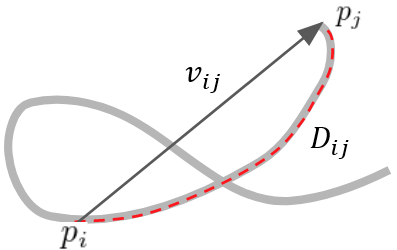
\includegraphics[width=2in]{method_geodesic}
    \caption{The length of the the red segment on the rope is the geodesic distance $\geodistIJ$. $\straightvecIJ$ is the vector showing the relative position of $\deformconfigJ$ with respect to $\deformconfigI$. \rev{Fix the notation in this image, considering moving Fig~\ref{fig:geodesic} here}}
    \label{fig:distance_vec_defs}
\end{figure}

The key assumption used by this method~\cite{Berenson2013} is \textit{diminishing rigidity}: the closer a gripper is to a particular part of the deformable object, the more that part of the object moves in the same way that the gripper does (i.e. more ``rigidly''). The further away a given point on the object is, the less rigidly it behaves; the less it moves when the gripper moves. In this section we refine Berenson's method by redefining $\JrotIG$ and introducing an extra parameter. This results in two parameters $\drktrans \geq 0$ and $\drkrot \geq 0$ which control how the translational and rotational rigidity scales with distance. Small values entail very rigid objects such as steel cable; high values entail very deformable objects such as fine string.

For every point $\deformidx$ and every gripper $\gripperidx$ we construct a Jacobian $\Jrigid(\deformidx, \gripperidx)$ such that if $\deformconfigI$ was rigidly attached to the gripper $\gripperconfigG$ then
\begin{equation}
    \deformvelI = \JrigidIG \grippervelG = 
    \begin{bmatrix} \JtransIG & \JrotIG \end{bmatrix} \grippervelG \enspace .
\end{equation}
We then modify this Jacobian to account for the effects of \textit{diminishing rigidity}. Let the indices of the set of points grasped by gripper $\gripperidx$ be $\GraspedPointsFull \subseteq \{1, \dots, \ndeformpoints \}$. Let $\closestpointIG$ be the index of the point with minimial relaxed geodesic distance to $\deformconfigI$ among the ones grasped by gripper $\gripperidx$:
\begin{equation}
    \closestpointIG = \argmin_{j \in \GraspedPointsFull} \geodistIJ \enspace .
\end{equation}
Then the translational rigidity of point $\deformidx$ with respect to gripper $\gripperidx$ is defined as
\begin{equation}
    \rigiditytransIG = e^{-\drktrans \geodistIG}
\end{equation}
and the rotational rigidity is defined as
\begin{equation}
    \rigidityrotIG = e^{-\drkrot \geodistIG}.
\end{equation}
To construct an approximate Jacobian $\tilde \Jacobian(\deformidx, \gripperidx)$ for a single point and a single gripper we combine the rigid Jacobians with their respective rigidity values
\begin{equation}
    \tilde \Jacobian(\deformidx, \gripperidx) = \begin{bmatrix} \rigiditytransIG \JtransIG & \rigidityrotIG \JrotIG \end{bmatrix} \enspace,
\end{equation}
and then combine the results into a single matrix
\begin{equation}
    \tilde \Jacobian(\gripperconfig, \deformconfig) = 
    \begin{bmatrix}
        \tilde \Jacobian(1,1) & \tilde \Jacobian(1,2) & \dots & \tilde \Jacobian(1, \ngrippers) \\
        \tilde \Jacobian(2,1) & \ddots \\
        \vdots \\
        \tilde \Jacobian(\ndeformpoints,1)
    \end{bmatrix} \enspace .
\end{equation}

%%%%%%%%%%%%%%%%%%%%%%%%%%%%%%%%%%%%%%%%%%%%%%%%%%%%%%%%%%%%%%%%%%%%%%%%%%%%%%%%%%%%%%%%%%%%%%%%%%%%%%%%%%%%%%%%%%%%%%%

\section{Constrained Directional Rigidity}
\label{sec:constrained_model}

\begin{figure}[t]
    \centering
    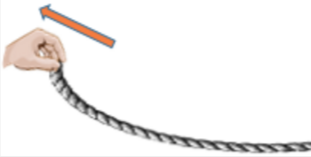
\includegraphics[width=.49\linewidth]{Intro_drag}\hfill
    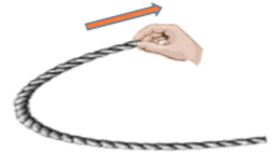
\includegraphics[width=.49\linewidth]{Intro_pull}%
    \caption{An illustrative example of directional rigidity. Left: The rope moves almost rigidly when dragging it by one end to the left. Right: The rope deforms when pulling it on the right in the opposite direction.}
    \label{fig:intro_directional_rigidity}
\end{figure}

While the diminishing rigidity Jacobian method has been used to do practical manipulation tasks with a deformable object~\cite{Berenson2013}, we observe that this rigidity does not only diminish as the distance from the gripper increases. Instead, it is a function of a larger set of variables derived from the configuration of the object. First, the rigidity also depends on the direction of gripper motion. Fig.~\ref{fig:intro_directional_rigidity} shows an example of an object's \textit{directional rigidity}. In addition capturing the effects of directional rigidity, in this section we seek to address contact with the environment, increasing the accuracy of the approximation.

\subsection{Model Overview}
% The approximate model locally describes the object's motion when given a motion of the grippers. Below we describe our approach first by specifying the model and then enforcing collision constraints on the prediction this model makes.

In Section~\ref{sec:diminishing_rigidity}, $\Jacobian$ is assumed to be independent of $\grippervel$ and $\obstacle$, yielding $\frac{\partial \DeformMapping}{\partial \gripperconfig} = \Jacobian(\gripperconfig, \robotconfighist, \deformconfig_0) = \Jacobian(\gripperconfig, \deformconfig)$, which is analogous to a rigid-body Jacobian. While these assumptions allow a linear relationship between $\grippervel$ and $\deformvel$, and thus computational convenience, they are not accurate in many situations (see Figure \ref{fig:intro_directional_rigidity} for an example). In this section we augment the definition of $\Jacobian$ to include effects from $\grippervel$ and $\obstacle$:
\begin{equation}
    \deformvel = \JacobianFull \grippervel = \DeformForwardFnFull \enspace .
\end{equation}

We now describe how $\Jacobian$ is approximated, focusing on how it accounts for directional rigidity (using $\grippervel$) and how it enforces obstacle penetration constraints (using $\obstacle$).

\subsection{Directional Rigidity}

We build on the idea proposed by Berenson~\cite{Berenson2013}, which approximates $\Jacobian$ based on the observation that the deformable object behaves rigidly near points grasped by the robot grippers. \cite{Berenson2013} encoded this effect through a simple function that only considered the distance of a point from the the nearest gripper. However, we find that we can exploit geometric information in the object's configuration to better predict the object's motion when we use a more complex model. We have observed that the key features of the deformable object configuration for predicting its motion are its deformability (which is determined by its material properties) and where it is slack. The deformation influences the transmission of the force from the grippers, i.e. the more stretchable the object, the more it will stretch when force is applied. However, when a region of the object is taut, regardless of how stretchable it is, it will move as if it were rigidly connected to a gripper (e.g. imagine a rope held taut by two grippers). We also must take into account that points are not influenced equally by different grippers, i.e. grippers farther away contribute less to the motion of a point than those closer to it.

To incorporate the above effects into our model, we define the following variables, which can be derived from $\gripperconfig, \grippervel$, and $\deformconfig$:
\begin{itemize}
    \item $\geodistIJ$: the geodesic distance (a scalar) between points $\deformconfigI$ and $\deformconfigJ$ on the surface of the object.
    \item $\straightvecIJ$: the vector starting at a point $\deformconfigI$ and ending at the point $\deformconfigJ$, as shown in Fig.~\ref{fig:distance_vec_defs}.
    \item $\gripperconfigG$: the configuration of gripper $\gripperidx$.
    \item $\grippervelG$: the velocity of gripper $\gripperidx$.
\end{itemize}

Furthermore, let $\closestpointIG$ be the index of the point with the minimal geodesic distance to $\deformconfigI$ among the ones grasped by the $\gripperidx$'th gripper. We address the notion of rigidity in object motion by considering the slackness of the object and reformulating the rigidity as a function of $\geodistIG$, $\straightvecIG$, and $\grippervelG$. For each point $\deformidx$ and gripper $\gripperidx$ we compute
\begin{equation}
\begin{split}
    \tilde \Jacobian(\deformidx, \gripperidx) 
                        &= \influenceIG \begin{bmatrix} \rigiditytransIG \JtransIG & \rigidityrotIG \JrotIG \end{bmatrix} \\
    \rigiditytransIG    &= \rigiditytrans(\geodistIG, \straightvecIG, \grippervelG) \\
    \rigidityrotIG      &= \rigidityrot(\geodistIG) \\
\end{split}
\label{eq:trans_rot_rigidity_diminishing_jacobian}
\end{equation}
$\rigiditytrans$ and $\rigidityrot$ are the corresponding translational and rotational diminishing rigidity factors defined by $\deformconfigI$ and gripper $\gripperidx$ (discussed below). 

Our goal is to encode the directional rigidity of the object motion into $\rigiditytrans$ and $\rigidityrot$ and use $\influenceIG$ to describe the \textit{influence} of gripper $\gripperidx$ on $\deformconfigI$. Intuitively, $\rigiditytrans$ should decrease with the increasing geodesic $\geodistIG$ distance between $\deformconfigI$ and $\deformconfigIG$. This is because the deformation of the region between $\deformconfigI$ and $\deformconfigIG$ will attenuate the transmitted force of the gripper's motion unless the object is taut. Since the effects on $\rigidityrotIG$ from $\grippervelG$ and $\straightvecIG$ are not as clear or significant as $\geodistIG$, we keep $\rigidityrotIG$ as a function of $\geodistIG$, where 
\begin{enumerate}
    \item $\rigidityrotIG$ ranges between $0$ and $1$.
    \item $\rigidityrotIG$ decreases as $\geodistIG$ increases.
\end{enumerate}
We give the definition of $\rigidityrotIG$ below.

From observation, we find two key reasons related to the slackness of the object that induce the diminishing rigidity effect for translation motion, and we aim to encode these factors into $\rigiditytransIG$. The first case is that the moving direction of $\grippervelG$ makes the region on the object between $\deformconfigI$ and $\deformconfigIG$ less taut. The second case is that this region is already slack. $\rigiditytransIG$ is thus a product of two terms:
\begin{equation}
    \rigiditytransIG = \tensionIG \slackIG
    \label{eq:Combined_directional_rigidity}
\end{equation}
where $\tensionIG$ addresses the effect in the first case (motion reducing tension), and $\slackIG$ addresses the effect in the second case (object slackness). Both $\tensionIG$ and $\slackIG$ are functions of some of $\gripperconfigG, \grippervelG, \deformconfigI$, or variables derived from these.

For $\deformconfigI$ on the object, we find $\tensionIG$ is greatly impacted by $\straightvecIG$ and $\transvelG$. Decomposing $\transvelG$ into $\transvelGRad$, the component in the direction of $\straightvecIG$, and $\transvelGPerp$, the component perpendicular to $\straightvecIG$. We observed that if $\transvelGRad$ is in the opposite direction to $\straightvecIG$, then it is more likely to make the intervening region slacker and thus reduce the transmission of force from the gripper to $\deformconfigI$. Moreover, if $\transvelGRad$ and $\straightvecIG$ are in the same direction when the object is not already slack, $\deformconfigI$ can move almost rigidly with $\grippervelG$. Fig.~\ref{fig:intro_directional_rigidity} shows an example of the impact of this alignment. Based on these observations, we design the function $\tensionIG = \tensionIGfull$ with the following properties:
\begin{enumerate}
    \item $\tensionIGfull$ ranges between $0$ and $1$.
    \item $\tensionIGfull > \tensionJGfull$
        \textbf{if} $\innerprod{\straightvecIG}{\transvelG} > \innerprod{\straightvecJG}{\transvelG}$
        \textbf{and} $\geodistIG = \geodistJG$.
    \item $\tensionIGfull > \tensionJGfull$
        \textbf{if} $\innerprod{\straightvecIG}{\transvelG} = \innerprod{\straightvecJG}{\transvelG}$
        \textbf{and} $\geodistIG > \geodistJG$.
\end{enumerate}
We give the definition of $\tensionIGfull$ below.


As mentioned above, $\slackIG$ depends on the current slackness of the intervening region. Without other external forces applied on the object, the pulling force applied by the robot will tend to unwind or unfold the object eventually (we do not consider cases where the object is tied into knots). For this reason,  the part of the intervening region on the object that is not already spread out is less likely to move rigidly with gripper $\gripperidx$. One indicator that can address this property is the ratio between the Euclidean distance between $\deformconfigI$ and $\deformconfigIG$, and the geodesic distance $\geodistIG$ between them. We denote $\distratioIG = \frac{||\straightvecIG||}{\geodistIG}$ to be this ratio. A larger $\distratioIG$ indicates a tauter intervening region. A tauter intervening region is more likely to result in $\deformvelI$ moving more rigidly. Thus we can design the function $\slackIG = \slackIGfull$ with the following properties:
\begin{enumerate}
    \item $\slackIGfull$ ranges between $0$ and $1$.
    \item $\slackIGfull = 1$ if $\distratioIG = 1$.
    \item $\slackIGfull > \slackJGfull$ if $\distratioIG > \distratioJG$
\end{enumerate}

Finally, $\influenceIG$, which captures the influence of gripper $\gripperidx$ on $\deformconfigI$ should have the following property (where $k$ is the index of a different gripper on the robot):
\begin{enumerate}
    \item $\influenceIG$ ranges between $0$ and $1$.
    \item $\influenceIG < \influenceIK$ if $\geodistIG > \geodistIK$.
    \item $\sum_{m = 1}^{\ngrippers} \influenceIM = 1$.
\end{enumerate}

Through experimentation, we obtained good results with the following functions:
\begin{equation}
\begin{split}
    \tensionIGfull  &= e^{\drkdir \geodistIG \left(\cos \angle \left( \straightvecIG, \transvelG \right) - 1\right)} \\
    \slackIGfull    &= \left( \frac{\| \straightvecIG \|}{\geodistIG} \right) ^{\drkdist} \\
    \rigidityrotIG  &= e^{-\drkrot \geodistIG} \\
    \influenceIG    &= \frac{x_\gripperidx}{\sum_{m = 0}^\ngrippers x_m}\\
    x_m             &= \frac{\textrm{min} \{\geodistI{1}, \dots , \geodistI{\ngrippers}\}}{\geodist_m} 
\end{split}
\label{eq:directional_rigidity_factors}
\end{equation}
where $\drkdir$, $\drkdist$, and $\drkrot$ are non-negative parameters. Specifically, a larger $\drkdir$ indicates a greater impact on the diminishing in the rigidity from the motion reducing tension. A larger $\drkdist$ indicates a greater impact on the diminishing in the rigidity from the slackness of the object in the current state. A larger $\drkrot$ indicates a faster decrease in rotational rigidity as the distance from $\deformconfigI$ to the gripper increases. 

\begin{figure}
    \centering
    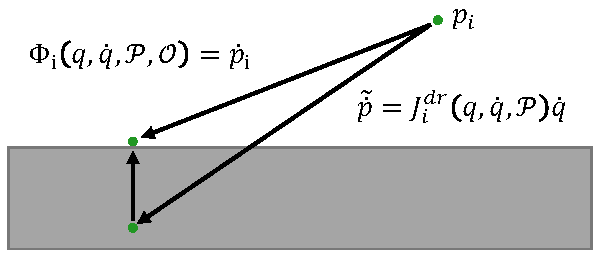
\includegraphics[width=3in]{point_projection}
    \caption{Projection process for points that are predicted to be in collision after movement.}
    \label{fig:point_projection}
\end{figure}

\subsubsection{Obstacle Penetration Constraints}

By combining the contributions of each individual gripper using the model developed above, we get a prediction of a point's movement from
\begin{equation}
    \approxPVI = \begin{bmatrix}
        \Jacobian(\deformidx, 1) & \dots & 
        \Jacobian(\deformidx, \ngrippers)
    \end{bmatrix} \grippervel = \Jacobian_{\deformidx}(\gripperconfig, \grippervel, \deformconfig) \grippervel
\end{equation}
However, at this stage, we haven't take into account the effect from the obstacles $\obstacle$. Thus the predicted $\approxPVI$ can move $\deformconfigI$ into an obstacle.

When the prediction of $\deformconfigI$ enters the obstacle, we project any penetration by the predicted $\approxPVI$ into the tangent space of the obstacle surface (Fig.~\ref{fig:point_projection}). Let $d_\deformidx < \| \approxPVI \|$ be the distance to collision in direction $\approxPVI$ from point $\deformconfigI$; let $\lambda_\deformidx = \frac{d_\deformidx}{\| \approxPVI \|}$; let $n_\deformidx$ be the unit surface normal of the obstacle in contact; and let $N_\deformidx = (\eye_{3\times 3} - \vec{n}_\deformidx \vec{n}_\deformidx^+)$. Then to account for obstacles we compute
\begin{equation}
    \tilde \Jacobian_\deformidx(\gripperconfig, \grippervel, \deformconfig, \obstacle) =
    \begin{cases}
        (\lambda_\deformidx + (1 - \lambda_\deformidx)N_\deformidx) \Jacobian_\deformidx(\gripperconfig, \grippervel, \deformconfig) & \text{if $\deformconfigI + \approxPVI$ in collision} \\
        \Jacobian_\deformidx(\gripperconfig, \grippervel, \deformconfig) & \text{otherwise}
    \end{cases}
\end{equation}
To generate $\Jacobian$ for all the points and grippers we compute $\Jacobian_\deformidx(\gripperconfig, \grippervel, \deformconfig)$ for each $\deformconfigI$. These matrices are modified using penetration constraints to get $\Jacobian_\deformidx(\gripperconfig, \grippervel, \deformconfig, \obstacle)$. These matrices are then stacked to obtain $\Jacobian(\gripperconfig, \grippervel, \deformconfig, \obstacle)$. Finally, we arrive at our approximate model: $\DeformForwardFnFull = \JacobianFull \grippervel$.

%%%%%%%%%%%%%%%%%%%%%%%%%%%%%%%%%%%%%%%%%%%%%%%%%%%%%%%%%%%%%%%%%%%%%%%%%%%%%%%%%%%%%%%%%%%%%%%%%%%%%%%%%%%%%%%%%%%%%%%

\section{Results}
\label{sec:modelling_results}

Our goal for the constrained directional regidity model is to improve the accuracy of the deformable object motion model (for use in the controller in Section~\ref{sec:stretching_constraint_controller}), while maintaing reasonable computation speed. Our benchmark model is the diminishing rigidity model described in Section~\ref{sec:diminishing_rigidity}. To evaluate our method we perform experiments in simulation and on a physical robot. The simulator used is Bullet physics \cite{Coumans2010}, however, we emphasize that our method has no knowledge of the simulation parameters or simulation methods used therein. The simulator is used as a ``black-box,'' mainly to stand in for a perception system and to allow us to do repeatable experiments. The physical robot consists of two KUKA iiwa 7DoF arms with Robotiq 3-finger hands.

We ran experiments with scenarios involving both cloth and rope. The parameters are set as $\drkdir = 4$, $\drkdist = 10$, $\drkrot = 20$ for the new model. The parameters we used for the benchmark method are its default best value found in \cite{Berenson2013}: $\drktrans = \drkrot = 10$ for rope and $\drktrans = \drkrot = 14$ for cloth. All experiments were run on a i7-8700K 3.7 GHz CPU with 32 GB of RAM. A video showing the experiments can be found at \url{https://www.youtube.com/watch?v=Y-wPsPdQVgg}.

\subsection{Simulation Environment Model Accuracy Results}

\begin{figure}[ht]
    \centering
    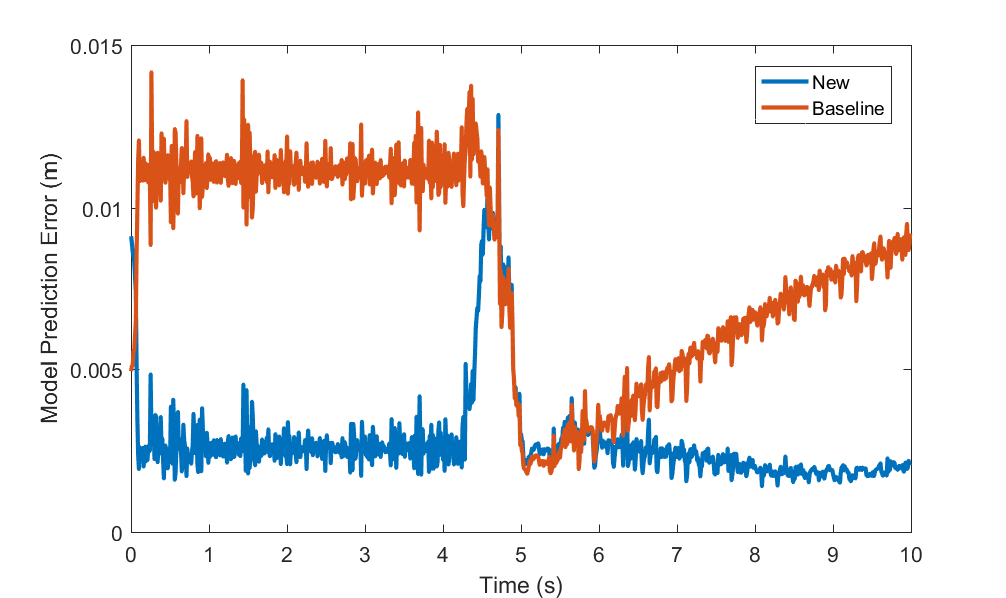
\includegraphics[width=0.85\columnwidth]{rope_model_accuracies}
    \caption{RMS model prediction error for the simulated rope model accuracy test. The gripper pulls the rope for the first 4.5 seconds, then turns for half a second, then moves in the opposite direction at the 5 second mark.}
    \label{fig:rope_model_accuracy_plot}
\end{figure}

\begin{figure}[ht]
    \centering
    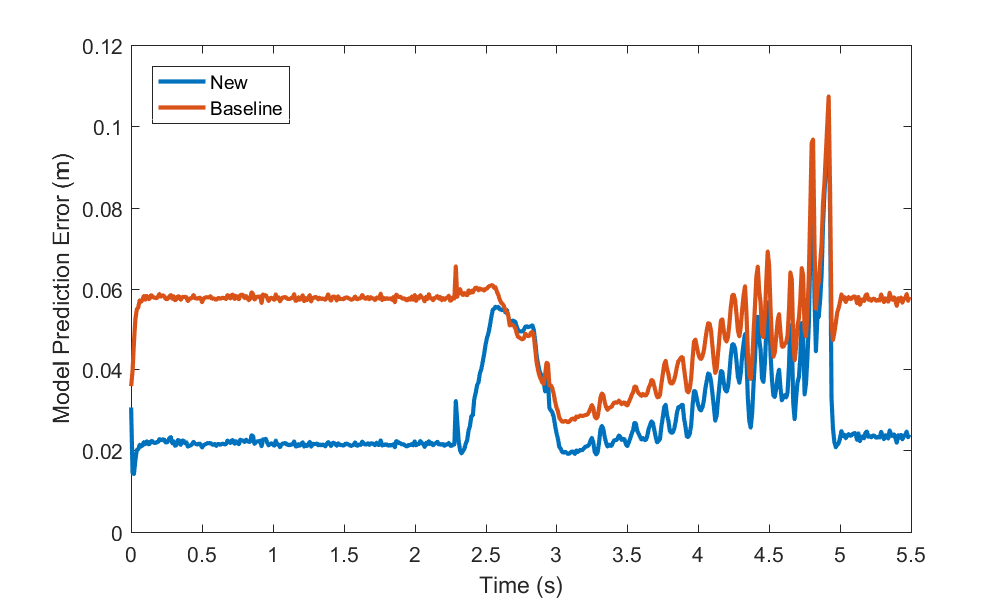
\includegraphics[width=0.85\columnwidth]{cloth_model_accuracies}
    \caption{RMS model prediction error for the simulated cloth model accuracy test. The grippers pull the cloth for the first 2.3 seconds, then turn for 0.63 seconds, then move in the opposite direction at the 2.93 second mark. At the 5 second mark the cloth is no longer folded. }
    \label{fig:cloth_model_accuracy_plot}
\end{figure}

We evaluated model accuracy by pulling the rope in a straight line along the direction of the rope, then turning the gripper and pulling back towards the rope as shown in Fig.~\ref{fig:intro_directional_rigidity}. As shown in Fig.~\ref{fig:rope_model_accuracy_plot}, our new model is a better approximation of the true motion when the gripper is pulling the rope. When the gripper is turning, both the baseline and the new model produce comparable error, but when the gripper starts pulling again (this time in the opposite direction), the new model is a significantly better approximation.

We also evaluated model accuracy by pulling the cloth in a similar fashion; pulling the cloth one way, turning the grippers, and then pulling in the opposite direction. As shown in Fig.~\ref{fig:cloth_model_accuracy_plot}, our new model is a better approximation of the true motion when the grippers are pulling the cloth. As in the rope test, when rotating the grippers both models produce comparable error. While the cloth is folded on itself both models produce noisy results, but when the cloth lies flat again, the new model achieves lower error.



\subsection{Physical Robot Experiments}

\begin{figure}[ht]
    \centering
    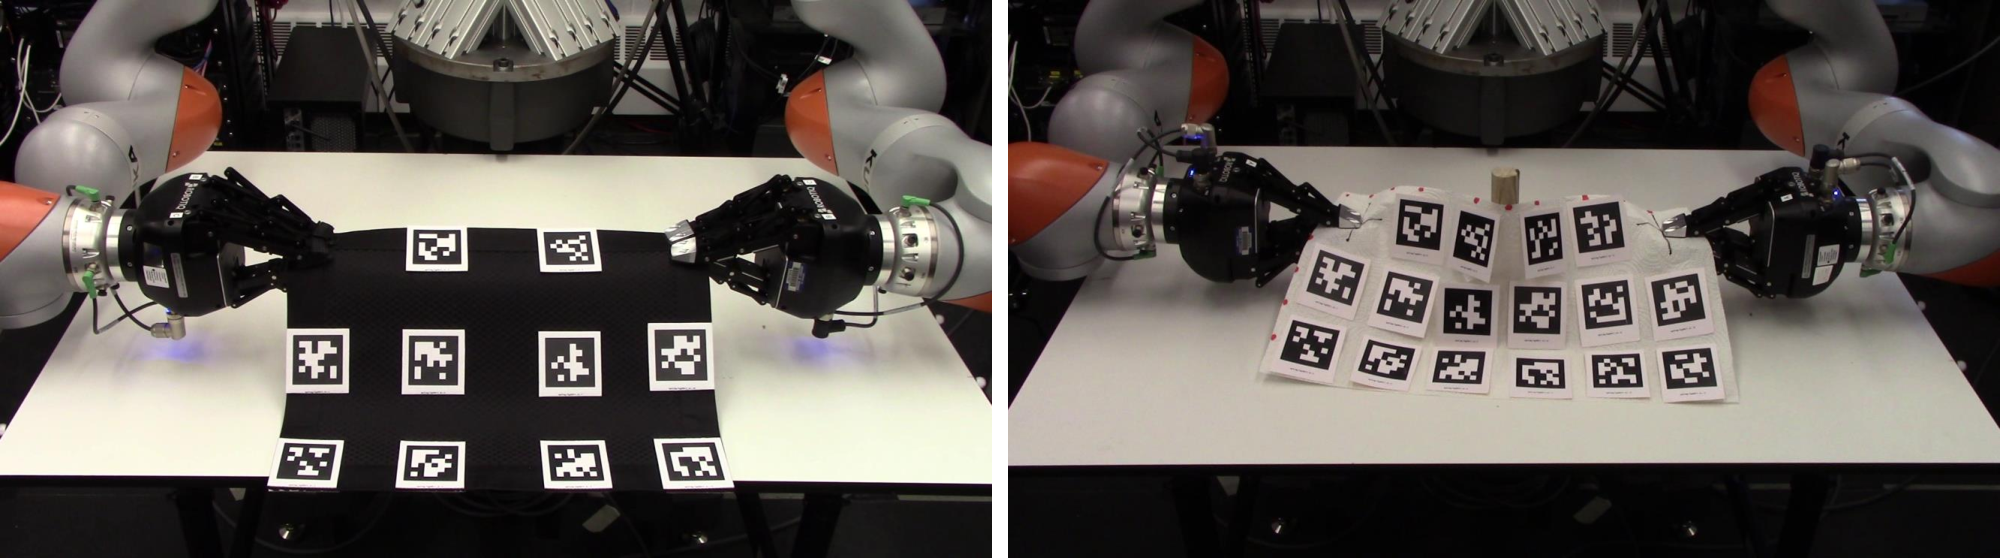
\includegraphics[width=.5\columnwidth,trim=0 0 6.7in 0,clip]{physical_robot_experiment_screenshots}
    \caption{Initial setup for the physical robot model accuracy experiment.}
    \label{fig:physical_experiment_screenshots}
\end{figure}

To evaluate our new model on a physical system, we set up an experiment with a cloth-like object manipulated by two 7DoF KUKA iiwa arms (Fig.~\ref{fig:physical_experiment_screenshots}). To sense the position of the cloth, we use the AprilTags~\cite{olson2011tags} and IAI Kinect2~\cite{iai_kinect2} libraries. The parameters are set as $\drkdir = 4$, $\drkdist = 10$, $\drkrot = 10$ for the new model. This test, which evaluates model accuracy, uses a motion profile similar to the simulation accuracy tests (Fig.~\ref{fig:cloth_model_accuracies_live}). Similar to the simulation results, the new model improves performance when dragging the cloth (first and last sections of Fig.~\ref{fig:cloth_model_accuracies_live}), and is comparable during rotational motion and when the cloth is resting on edge perpendicular to the table (see video).

\begin{figure}[ht]
    \centering
    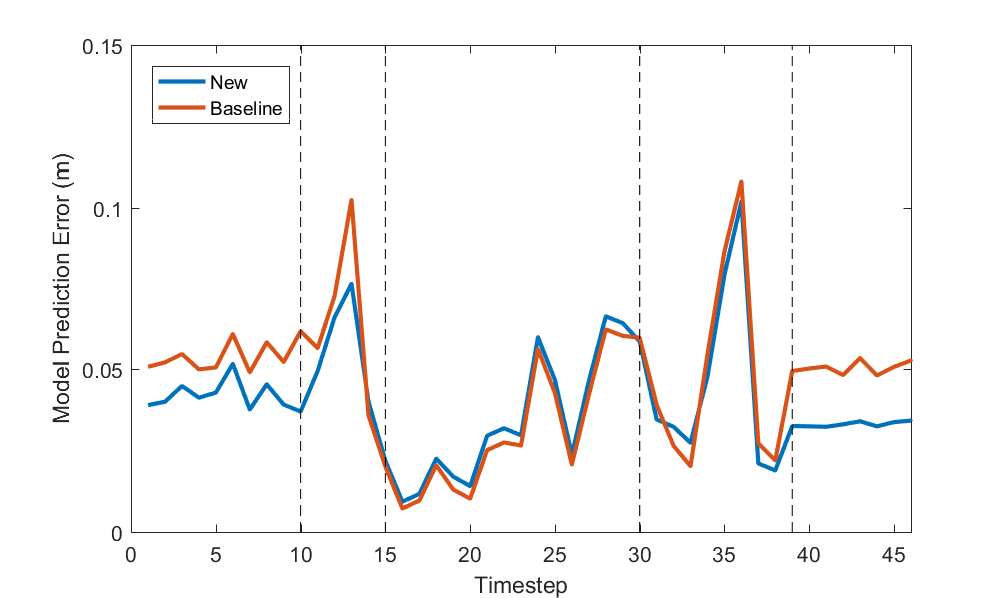
\includegraphics[width=\columnwidth]{cloth_model_accuracies_live.png}
    \caption{RMS model prediction error. The grippers pull the cloth toward the robot for the first 10 timesteps, upward for 5 timesteps, rotate for 15 timesteps, diagonally down and away for 9 timesteps, then directly away from the robot.}
    \label{fig:cloth_model_accuracies_live}
\end{figure}

\subsection{Computation Time}

\begin{figure}[t]
    \centering
    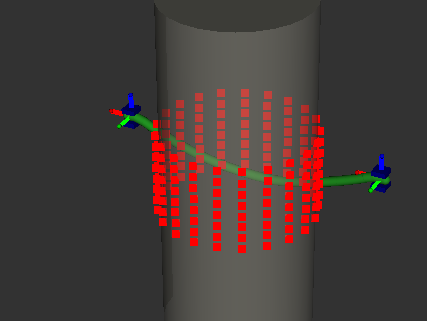
\includegraphics[width=.45\linewidth]{rope_cylinder}\hfill
    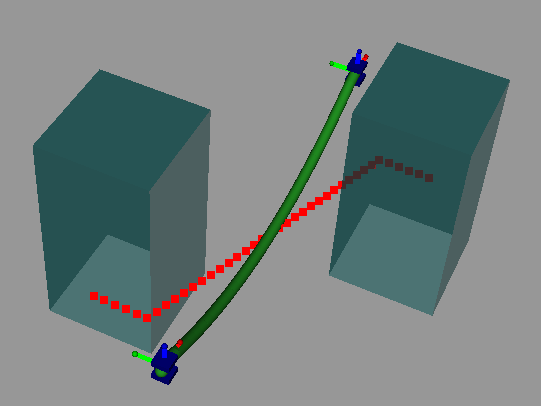
\includegraphics[width=.45\linewidth]{rope_zig_match}\\
    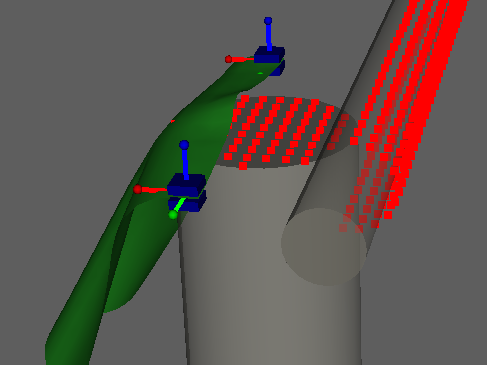
\includegraphics[width=.45\linewidth]{cloth_wafr}\hfill
    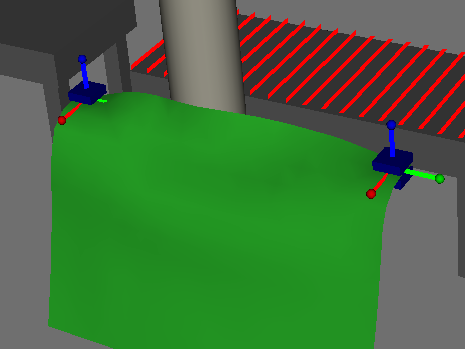
\includegraphics[width=.45\linewidth]{cloth_single_pole}%
    \caption{Initial state of four experiments for model computation time tests, where the red points act as attractors for the deformable object. TL: rope-wrapping-cylinder; TR: rope-matching-zig-path; BR: cloth-passing-single-pole: BL: cloth-wrapping-two-cylinders.}
    \label{fig:modelling_timing_tests}
\end{figure}


\begin{table}[ht]
\centering
\caption{Top two rows: Mean computation time (ms) per model prediction for a given gripper motion. BT: Bullet simulator; CDR: constrained directional rigidity. Bottom row: Mean number of times the model was evaluated when executing the controller in Section~\ref{sec:stretching_constraint_controller}.}
\label{tbl:simulation_time_report}
\begin{tabular}{ccccc}
\hline
            & \makecell{rope-wrapping\\-cylinder} 
            & \makecell{rope-matching\\-cylinder}
            & \makecell{cloth-passing\\-single-pole}
            & \makecell{cloth-wrapping\\-two-cylinder} \\
\hline
BT          & 0.686 & 0.571 & 19.29 & 3.680 \\
CDR         & 0.029 & 0.014 & 1.172 & 0.339 \\
\hline
\# evals    & 50.72 & 143.5 & 83.81 & 63.32 \\
\hline
\end{tabular}
\end{table}

To verify the practicality of our method, we gathered data comparing its computation time to the benchmark's and to using the Bullet simulator for a variety of tasks (see Fig.~\ref{fig:modelling_timing_tests} and Section~\ref{sec:stretching_constraint_controller_results}). Table~\ref{tbl:simulation_time_report} shows a comparison between the average time needed to evaluate the new model and the time needed to simulate a gripper motion with the Bullet simulator. Note that the amount of time required for the simulator to converge to a stable estimate depends on many conditions, including what object is being simulated. Through experimentation we determined that 4 simulation steps were adequate for rope and 10 for cloth. Comparing the time needed to do this simulation to the time needed to evaluate our model, we see that the new model is indeed faster by at least an order of magnitude, in some cases by two orders of magnitude, confirming that, despite being slower than the diminishing rigidity model, our method still outperforms the simulator in terms of computation time. This is particularly important given the average number of times a model is evaluated in a control loop.
